\documentclass{beamer}
\usepackage[utf8]{inputenc}
\usepackage{palatino}
\usepackage{listings} %Allows including source code
\usepackage{graphicx} % Allows including images
\usepackage{booktabs} % Allows the use of \toprule, \midrule and \bottomrule in tables
%\usepackage{bookman}
%\usepackage{courier}
% For more themes, color themes and font themes, see:
% http://deic.uab.es/~iblanes/beamer_gallery/index_by_theme.html
%
\mode<presentation>
{
	\usetheme{Madrid}       % or try default, Darmstadt, Warsaw, ...
	\usecolortheme{default} % or try albatross, beaver, crane, ...
	\usefonttheme{serif}    % or try default, structurebold, ...
	\setbeamertemplate{navigation symbols}{}
	\setbeamertemplate{caption}[numbered]
} 
\usepackage{listings}
\usepackage{color}

\definecolor{codegreen}{rgb}{0,0.6,0}
\definecolor{codegray}{rgb}{0.5,0.5,0.5}
\definecolor{codepurple}{rgb}{0.58,0,0.82}
\definecolor{backcolour}{rgb}{0.95,0.95,0.92}

\lstdefinestyle{mystyle}{
	%backgroundcolor=\color{backcolour},   
	%commentstyle=\color{codegreen},
	commentstyle=\itshape\color{green!40!black},
	keywordstyle=\bfseries\color{blue},
	numberstyle=\tiny\color{black},
	stringstyle=\color{purple},
	basicstyle=\footnotesize,
	breakatwhitespace=false,         
	breaklines=true,                 
	captionpos=b,                    
	keepspaces=true,                 
	numbers=left,                    
	numbersep=5pt,                  
	showspaces=false,                
	showstringspaces=false,
	showtabs=false,                  
	tabsize=2
}

\lstset{style=mystyle}
\title[Software Engineering] %optional
{Software Engineering}

\subtitle{Introduction to UML}

\author[SOUM Somon] % (optional, for multiple authors)
{SOUM Somon}

\institute[Bc.CS] % (optional)
{ Institute of Technology of Cambodia }

\date[SE 2017] % (optional)
{Semister II, April 2017}

\logo{
\includegraphics[height=1.5cm]{Uml_logo.png}}
\begin{document}
	\begin{frame}
		\titlepage % Print the title page as the first slide
	\end{frame}
	\begin{frame}
		\frametitle{Table of Contents} % Table of contents slide, comment this block out to remove it
		\tableofcontents % Throughout your presentation, if you choose to use \section{} and \subsection{} commands, these will automatically be printed on this slide as an overview of your presentation
	\end{frame}
%----------------------------------------------------------------------------------------
%	PRESENTATION SLIDES
%----------------------------------------------------------------------------------------

%------------------------------------------------
\section{Introduction} % Sections can be created in order to organize your presentation into discrete blocks, all sections and subsections are automatically printed in the table of contents as an overview of the talk
%------------------------------------------------
\begin{frame}{What is UML?}
	\begin{enumerate}
		\item UML is short for Unified Modeling Language
		\item UML is the standard modeling language for software\\
		and systems development
		\item It consists of an integrated set of diagrams developed\\
		to help accomplish the following tasks:
			\begin{itemize}
				\item<1-> Specification
				\item<2-> Visualization
				\item<3-> Architecture design
				\item<4-> Construction
				\item<5-> Simulation and Testing
				\item<6-> Documentation
			\end{itemize}
		
	\end{enumerate}
\end{frame}

\section{What’s in a Modeling Language?}
		\begin{frame}
			\frametitle{What’s in a Modeling Language?}
			\begin{itemize}
				\item 6 main advantages of UML
				\begin{enumerate}
					\item It’s a formal language
					\item  It’s concise
					\item It’s comprehensive
					\item It’s scalable
					\item It’s built on lessons learned
					\item It’s the standard
				\end{enumerate}
			\item Detailed Overload: Modeling with Code
				\begin{example}
				Software code is an example of a potential modeling language where none of the detail has been abstracted
				away. Every line of code is the detail of how your software is intended to work. This example shows a very
				simple class in Java, yet there are many details in this declaration.
				\end{example}
			\end{itemize}
		\end{frame}
		\begin{frame}{What’s in a Modeling Language?}
			\begin{example}
			\lstinputlisting[language=Java]{Guitarist.java}
			\end{example}
	\end{frame}
	\begin{frame}{What’s in a Modeling Language?}
		\begin{enumerate}
		\item Verbosity, Ambiguity, Confusion: Modeling with
			Informal Languages
			\begin{figure}
				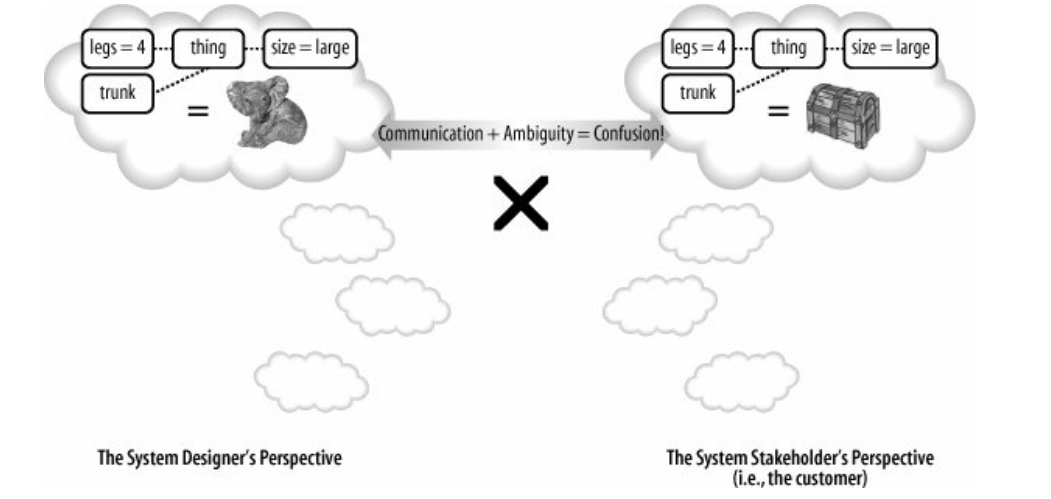
\includegraphics[width=0.90\textwidth]{img1}
				\caption{With an informal notation, the problem of confusion \newline through ambiguity still exists}
			\end{figure}
	\end{enumerate}
\end{frame}
	\section{Models and Diagrams}
		\begin{frame}{Models and Diagrams}
		\end{frame}
	\section{Views of Your Model}
		\begin{frame}{Views of Your Model}
			
		\end{frame}
	\section{Dispelling Misconceptions about UML}
		\begin{frame}{Dispelling Misconceptions about UML}
			
		\end{frame}
\end{document}